\documentclass[11pt, a4paper]{article}
\usepackage[utf8x]{inputenc}
\usepackage[english]{babel}
\usepackage[T1]{fontenc}
\usepackage{mathptmx}

\usepackage[pdftex]{graphicx}
\usepackage[pdftex, linkcolor=black, pdfborder={0 0 0}]{hyperref}
\usepackage{calc}
\usepackage{enumitem}
\usepackage{indentfirst}

\frenchspacing
\linespread{1.2}
\usepackage[a4paper, lmargin=0.2\paperwidth, rmargin=0.2\paperwidth, tmargin=0.1\paperheight, bmargin=0.1\paperheight]{geometry}

\usepackage[all]{nowidow}
\usepackage[protrusion=true,expansion=true]{microtype}

\begin{document}

\begin{titlepage}
   \vspace*{\stretch{1.0}}
   \begin{center}
      \Large\textbf{Project Proposal: Detection, tracking and location of runways on visual approaches}\\
      \large\textit{Daniel Benvenutti 169448, Matteo Di Fabio 264339 and Renan Sterle 176536}
   \end{center}
   \vspace*{\stretch{2.0}}
\end{titlepage}

\section{Introduction and Motivation}

	Both in military aviation as well as in civil aviation, visual flight rules (VFR) remain of great importance nowadays. Particularly in airports and terminals of reduced infrastructure, visual approach and landing procedures account for the majority of cases and such procedures rely on visibility conditions, visual navigational aids and personal performance of the pilot in command. Figure \ref{fig:Approach} depicts what a final visual approach looks like.

	In any type of landing approach, the maintenance of a safe flight envelope is crucial. Therefore, during the final approach leg, parameters such as airspeed, altitude, descent rate, glide slope, ground clearance, as well as location in relation to the runway must be monitored and corrected.

	While airspeed, altitude and descent rate are measure by the aircraft, the other parameters can only be determined with the use of external information. In the case of instrument flight rules (IFR), Instrument Landing Systems (ILS), Global Navigation Satellite System (GNSS), inertial navigation systems and radio beacons provide such information, whereas on VFR they are ultimately estimated visually by the pilot.

	The idea of this project is to implement a system that:

	\begin{enumerate}
		\item Given a picture of an approach, identifies and isolates the runway in question, using image processing filtering and segmentation techniques, as seen in Figure \ref{fig:Segmented};
		\item Fits the runway image into the expected runway shape by applying perspective and affine transformations, as seen in Figure \ref{fig:Runway};
		\item Determines the camera point of view in relation to the runway start. Alignment, lateral offset and distance information are the most important, while relative altitude is of secondary importance;
		\item Tracks the identified runway in a stream of frames, validating and checking the correlation of the results between different frames of a temporal sequence;

	\end{enumerate}
	
\begin{figure}[htp]
    \centering
    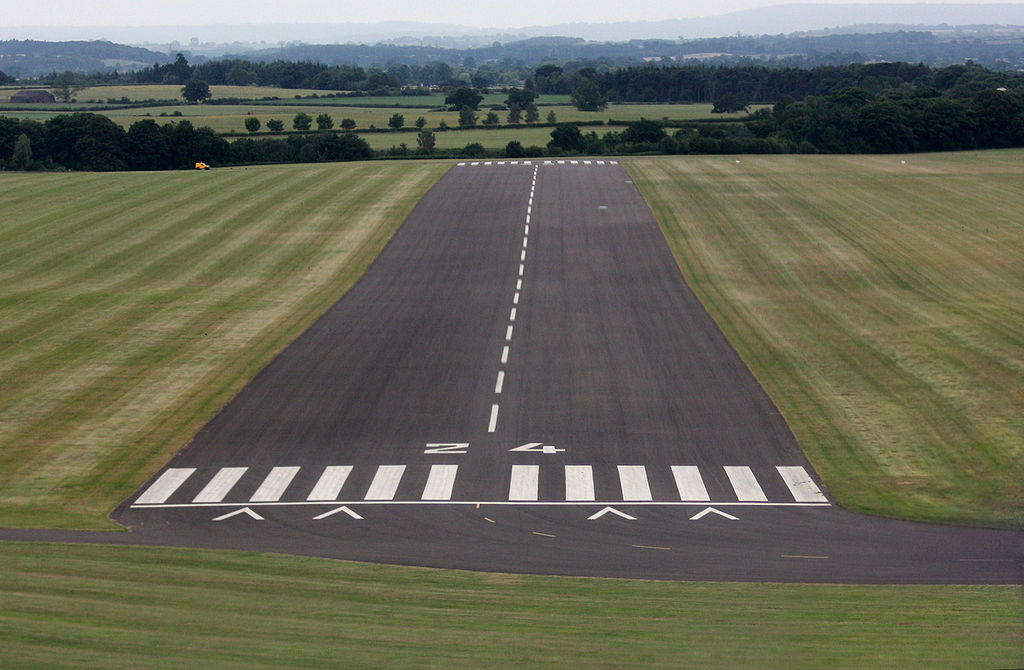
\includegraphics[width=6cm]{Images/Approach.jpg}
    \caption{Approach view.}
    \label{fig:Approach}
\end{figure}

\begin{figure}[htp]
    \centering
    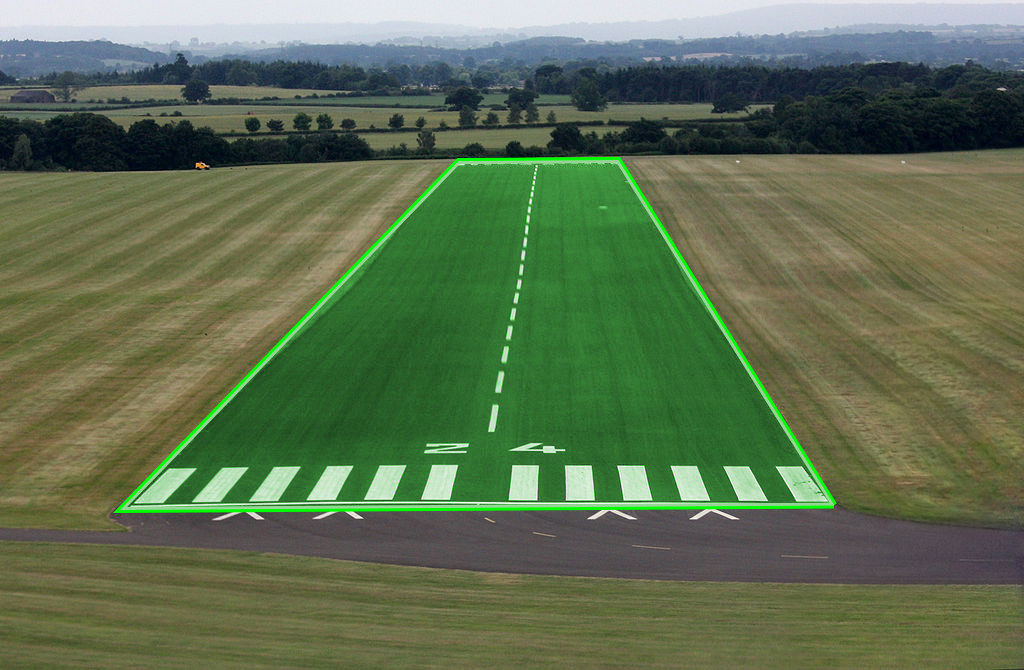
\includegraphics[width=6cm]{Images/Segmented.jpg}
    \caption{Segmented runway.}
    \label{fig:Segmented}
\end{figure}

\begin{figure}[htp]
    \centering
    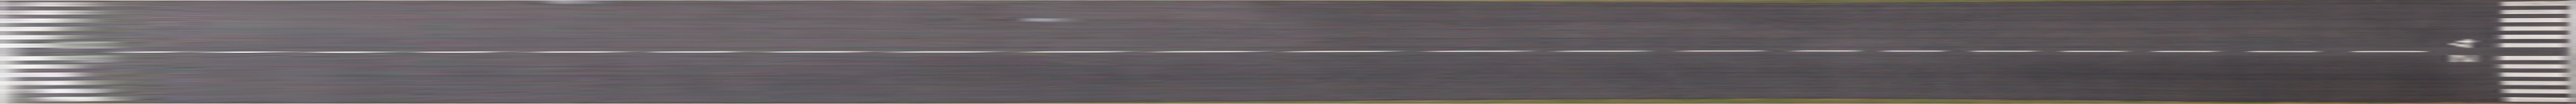
\includegraphics[width=10cm]{Images/Runway.jpg}
    \caption{Retrieved runway image.}
    \label{fig:Runway}
\end{figure}

\section{Theoretical Background}

	Most landing runways are approximately flat. Therefore, when photographed in two dimensions from a different plane in the 3D space, they can be encapsulated within a quadrilateral. This quadrilateral can be mapped to the expected rectangular 2D shape of the runway with perspective and affine transformations as in \cite{Paper}. Therefore, the coordinates of the camera can be determined in terms of those of the runway, and so can the relevant aeronautical parameters.

\section{Proposed Development Plan}

	The project can be developed in several independent fronts simultaneously with a final merge and constitution of the full pipeline. Tasks such as:
	
	\begin{enumerate}
		\item Finding the runway;
		\item Isolating and correcting projection of runway;
		\item Given a runway's bounding quadrilateral in the image, find finding camera's point of view;
		\item Given camera's position, calculating the relevant parameters;
		\item Validating the obtained parameters by comparison to the sequential temporal series in the case of a video stream;
	\end{enumerate}

\section{Data Source}

	As data sources, there is plenty of video footage of landings from the cockpit point of view on YouTube and similar platforms. Also, more standardized footage can be generate on purpose and in controlled manner with the use of flight simulators.

\section{Evaluation}

	For evaluation purposes, along with qualitative functionality of the system, a few metrics can be defined for a quantitative analysis. For example, one can determine for which visibility conditions the runway is correctly detected, from which distance and with which derivation between frames. Also, data from a flight simulator can be generated so that the real parameters can be known and compared to the calculated ones. Thus, the error margins can be explicitly determined.

\begin{thebibliography}{1}
\bibitem{Paper} 
Estrems Amestoy, Manuel/de Francisco Ortiz, Óscar (2019): Global Positioning from a Single Image of a Rectangle in Conical Perspective, in: Sensors, Heft 24 (19) 10.12.2019, S. 5432, URL: http://dx.doi.org/10.3390/s19245432.
\end{thebibliography}

\end{document}